\section{Systematic uncertainty}
\label{sec:syst}

The main experimental uncertainties which affect both signal and background are the uncertainty on the integrated luminosity
(2.6\% for 2016~\cite{CMS-PAS-LUM-17-001}, 2.3\% for 2017~\cite{CMS-PAS-LUM-17-004}, XX\% for 2018) and the uncertainty on the lepton 
identification and reconstruction efficiency (ranging from 2.5--9\% on the overall event yield for the $4\mu$ 
and $4e$ channels, respectively). 

The uncertainty on the lepton energy scale is determined by considering the 
$Z\rightarrow\ell\ell$ mass distributions in data and simulation. Events are separated into categories based on the 
$\pt$ and $\eta$ of one of the two leptons, determined randomly, and integrating over the other. The dilepton mass 
distributions are then fit to a Breit-Wigner 
parameterization convolved with a double-sided Crystal Ball function. The offset in the measured peak position with 
respect to the nominal $\cPZ$ boson 
mass in data and simulation are extracted, and the results are shown in Fig.~\ref{fig:lepScale_16}. The relative difference 
between data and simulation is propagated to the reconstructed \mass{Z2} distribution 
for signal and background events 
The uncertainty is determined to be 0.04\% (0.3\%) for the  $4\mu$ ($4\Pe$) channels, respectively. 

Experimental uncertainties for the reducible background estimation, described in Section~\ref{sec:redbkgd},
vary between XX\% ($4\mu$) to XX\% ($4e$).

\begin{figure}[!htb]
\begin{center}
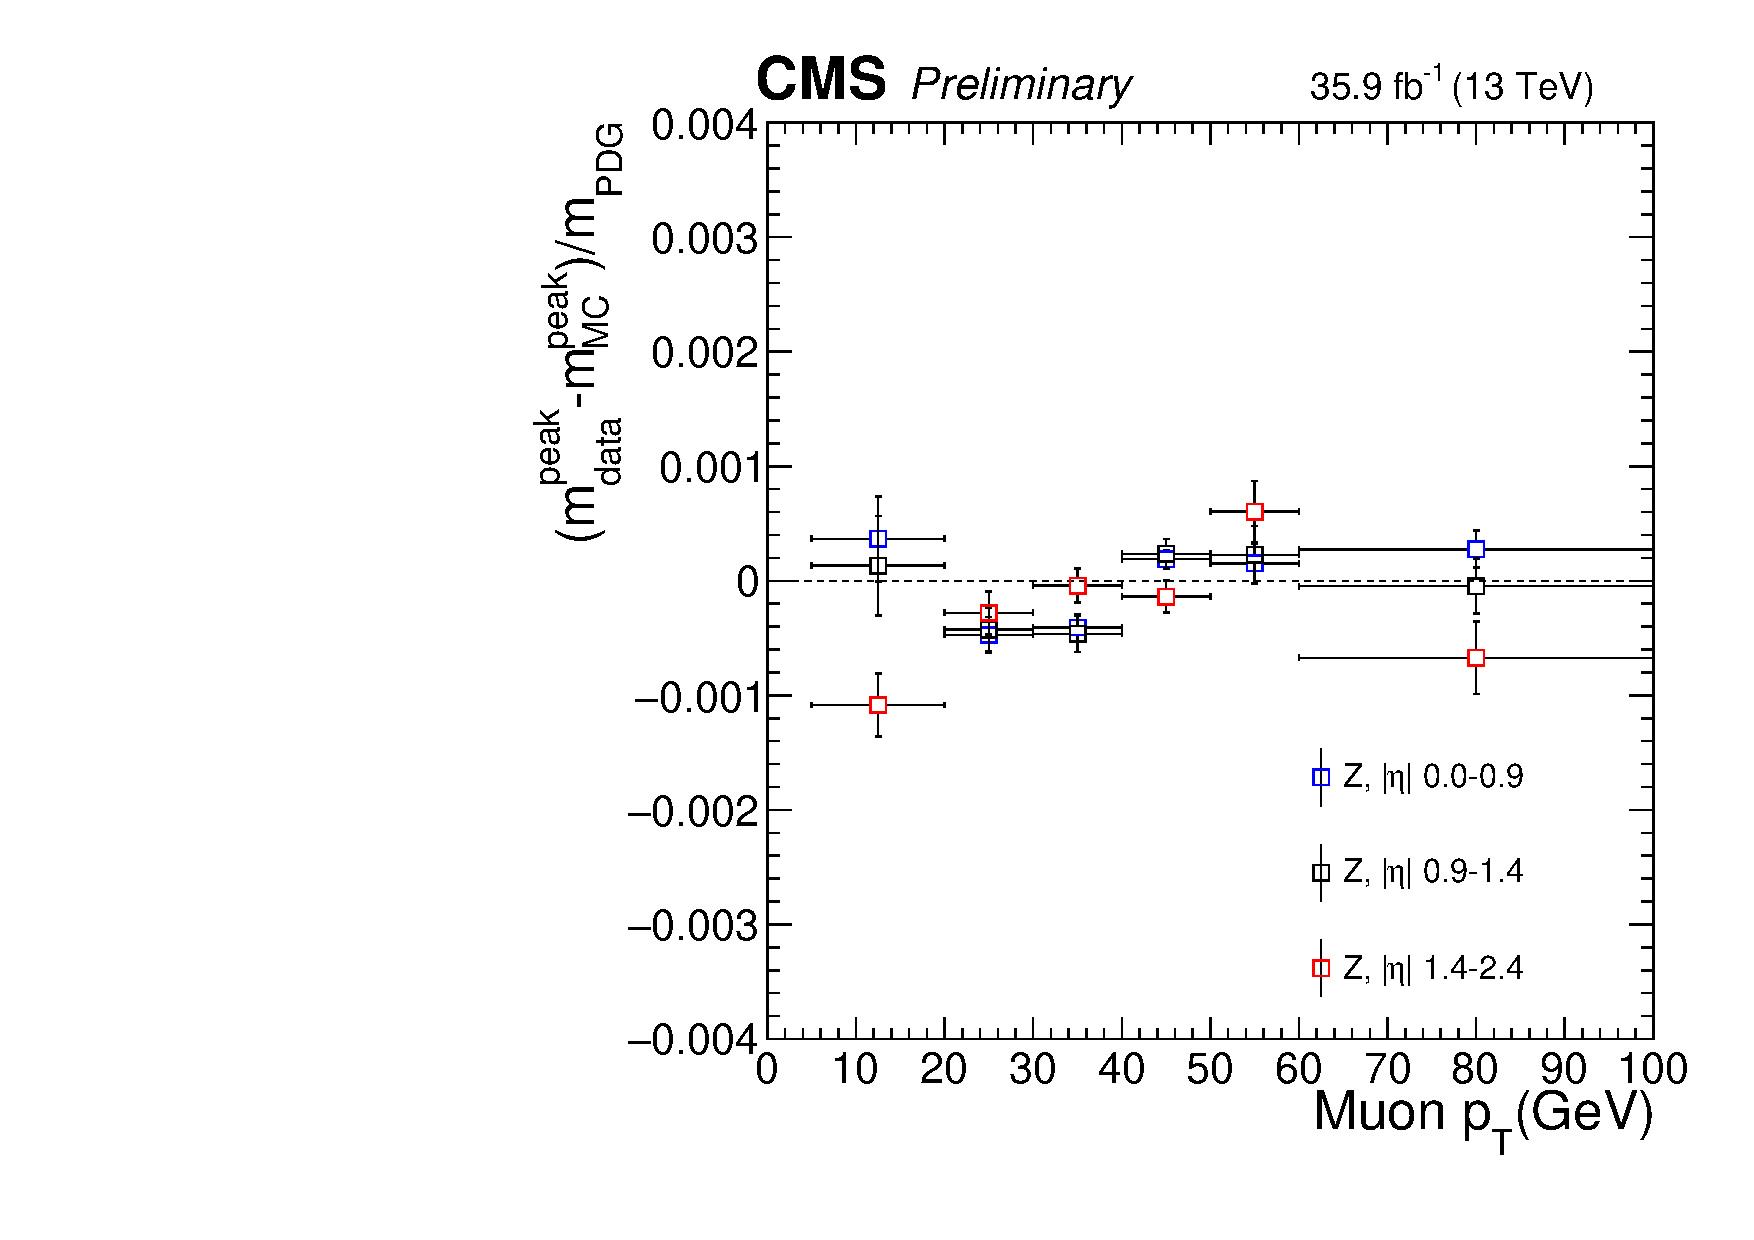
\includegraphics[width=0.44\linewidth]{Figures/Systematic/mass/lepScale_vs_pt_eta_mu.pdf}
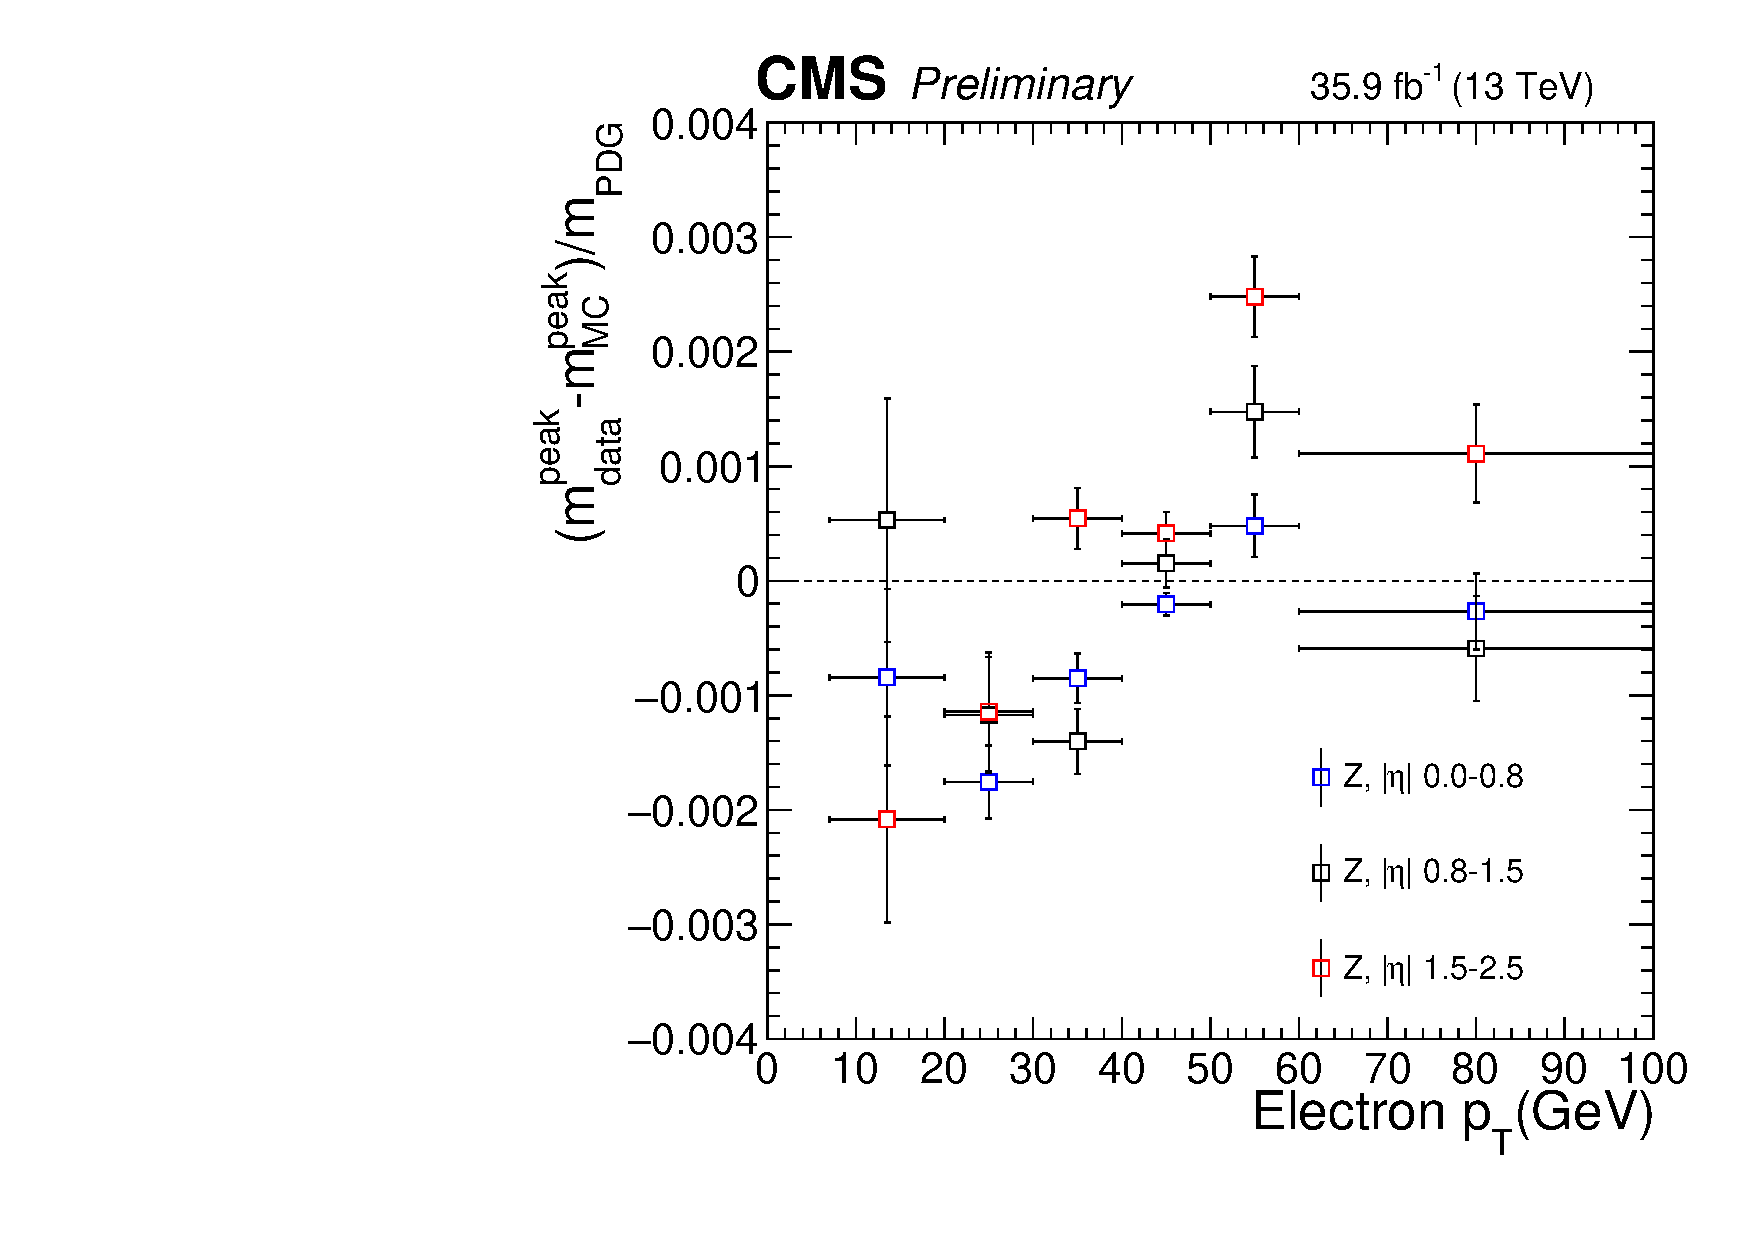
\includegraphics[width=0.44\linewidth]{Figures/Systematic/mass/lepScale_vs_pt_eta_e.pdf}
\caption{ Difference between the ${\rm Z}\rightarrow\ell\ell$ mass peak positions in data and simulation normalized by the 
nominal $\cPZ$ boson mass obtained as a function of the $\pt$ and $|\eta|$ of one of the leptons regardless of the second
for muons (left) and electrons (right).
\label{fig:lepScale_16}}
\end{center}
\end{figure}

Theoretical uncertainties which affect both the background signal and background estimation 
include uncertainties from the renormalization and factorization scale and choice of PDF set. 
The uncertainty from the renormalization and factorization scale is determined by varying these scales between 
0.5 and 2 times their nominal value while keeping their ratio between 0.5 and 2. 
The uncertainty from the PDF set is determined 
by taking the root mean square of the variation when using different replicas of the default NNPDF set. An additional
uncertainty of the 10\% on the K factor used for the $\ggZZ$ prediction is applied as described in Section~\ref{sec:irrbkgd}.
A systematic uncertainty of 2\% on the branching ratio of $\HZZfl$ only affects the signal yield. 

\begin{table}[!htb]
\begin{center}
\small
\caption{
Summary of the experimental systematic uncertainties in the $\Hllll$ measurements. %Details about the derivation of each uncertainty can be found in the text.
\label{tab:SystOverview}
}
\begin{tabular}{|lc|} 
\hline %---------------------------------------------------------
\hline %---------------------------------------------------------
\multicolumn{2}{|c|}{\textbf{Summary of relative systematic uncertainties}} \\
\hline %---------------------------------------------------------
\hline %---------------------------------------------------------
\multicolumn{2}{|c|}{Common experimental uncertainties} \\
\hline %---------------------------------------------------------
\vspace{-0.4cm} & \\
Luminosity & 2.6 \%  \\ 
\vspace{-0.4cm} & \\
Lepton identification/reconstruction efficiencies & 2.5 -- 9 \% \\ 
\vspace{-0.4cm} & \\
Lepton energy scale & 0.04 -- 0.3 \% \\ 
\vspace{-0.4cm} & \\
Lepton energy resolution & 20 \% \\ 

\hline %---------------------------------------------------------
\hline %---------------------------------------------------------
\multicolumn{2}{|c|}{Common theory related uncertainties} \\
\hline %--------------------------------------------------------
\vspace{-0.4cm} & \\
Higgs branching fraction & 2 \% \\
\vspace{-0.4cm} & \\
QCD scale & 0.4 -- 4.2 \% \\
\vspace{-0.4cm} & \\
PDF scale & 1.6 -- 3.4 \% \\
\vspace{-0.4cm} & \\
Reducible background (Z+X) & XX -- XX \% \\ 
\hline %---------------------------------------------------------
\hline %---------------------------------------------------------
\multicolumn{2}{|c|}{Background related uncertainties} \\
\hline %--------------------------------------------------------
\vspace{-0.4cm} & \\
Reducible background (Z+X) & XX -- XX \% \\ 
\vspace{-0.4cm} & \\
\qqZZ electroweak correction & 0.1 \% \\
\vspace{-0.4cm} & \\
\ggZZ kfactor & 10.0 \% \\
\hline %---------------------------------------------------------
\hline %---------------------------------------------------------
\multicolumn{2}{|c|}{Signal related uncertainties} \\
\hline %---------------------------------------------------------
Interference & 5.0 \% \\ 
\vspace{-0.4cm} & \\
Higher order correction & TBD \% \\
\vspace{-0.4cm} & \\
Signal branching fraction & TBD \% \\
\hline %---------------------------------------------------------
\hline %---------------------------------------------------------
\end{tabular}
\normalsize
\end{center}
\end{table}
